\chapter{Server-Virtualisierung}

\section{Grundlagen}
Überall kann man Virtualisierung einsetzen. Ob bei Server, Speicher, Applikation, Desktops oder Netzwerk. Mit Virtualisierung will man die Abstraktion von der darunterliegende Gerätschaft erreichen.

\subsection{Virtualisierungsarten}
\begin{description}
	\item[HW Partitionierung] Teuer, nur noch auf High End Computer anzutreffen, wie IBM/z, und p Systems, Sun/Oracle Sparc).
	\item[HW Virtualisierung] Mittels Hypervisor.
	\item[OS Virtualisierung] Jung, leichtgewichtig Virtualisierungsart. 
\end{description}

\subsection{Gründe für eine HW Virtualisierung}
\begin{itemize}
	\item Ressourcen Optimierung
	\item Konsoldierung
	\item Maximierung der Uptime
	\item Schutz der Applikation von Serverausfällen
	\item Einfache Migration wenn Anforderungen wechseln
	\item Schutz der Investitionen in existierende ''legacy Systeme'' 
\end{itemize}

\subsection{Geschichte}
IBM virtualisiert auf den Mainframes bereits in den 60er Jahren. Die Virtualisierung der x86-Systeme wurde erst 1999 eingeführt, durch VMWare. Citrix hat 2007 mit Xen/Xen-Server virtualisiert und Mircosoft im 2008 mit Window Server 2008 und Hyper-V.

\subsection{Was bedeutet Virtualisierung?}
Darüber streiten sich Joho und die Geister. Was ist Emulation? Simulation? Imitation?  Virtualisation?
\begin{description}
	\item[Emulation] Ein System ahmt ein anderes System nach. Es bekommt den selben Input. Die Verarbeitung wird emuliert. Das führt dazu, dass der Output gleich oder nur fast gleich ist.
	\item[Simulation] Zu Grunde liegt ein Modell, welches die Schlüssel-Charakteristika des zu Simulierenden repräsentiert.
	\item[Virtualität] Eigenschaft einer Sache, nicht in der Form zu existieren, in der sie zu existieren scheint.
	\item[Virtualisierung] Bezieht sich auf den Vorgang der Erstellung einer virtuellen (nicht tatsächlich existenten) Version von etwas. Beispiel: Computer-Hardware, OS, Speichergeräte, Computer-Netzwerk-Ressourcen. 
\end{description}

\subsection{Die drei Anforderungen von Popek und Goldberg}
Diese Anforderungen gelten sowohl ans physische wie auch virtuelle System.
\begin{description}
	\item[Gleichheit] Jedes Programm verhält sich auf deinen Systemen genau gleich. Wichtig!
	\item[Effektivität] Es soll, wann immer möglich, alle Instruktionen direkt auf dem physischen Prozessor ausgeführt werden. Ohne Intervention der VMM.
	\item[Ressourcenkontrolle] VMM hat die komplette Kontrolle über Ressourcen wie Memory, I/O der Peripheriegeräte, aber nicht umbedingt über Prozessoraktivität. Es muss für jedes Programm unmöglich sein die System Ressourcen (wie verfügbares Memory) zu beeinflussen. Der Verteiler (Allocator) muss jedesmal aufgerufen werden.
\end{description}

\subsection{VMM - Virtual Machine Mointor}
\begin{figure}[h!]
	\centering
	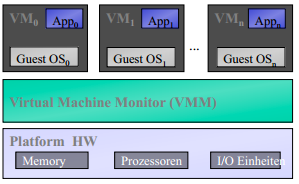
\includegraphics[width=0.4\linewidth]{fig/vmm}
	\caption{VMM}
	\label{fig:vmm}
\end{figure}
Die VM ist die Umgebung erzeugt vom VMM. Die VMM ist eine System Software Schicht und besteht aus folgenden drei Teilen:
\begin{description}
	\item[Dispatcher] dessen Initial Instruction am Speicherplatz liegt wohin die HW trapped.
	\item[Allocator] der entscheidet wer welche Systemressourcen bekommt. Er hat 1 oder n Member (VM).
	\item[Interpreter] für alle Instruktionen die trappen, eine Interpreter Routine pro privilegierte Instruktion.
\end{description}

\subsection{Instruktionsklassifikation}
Es gibt zwei Betriebsmodis.
\begin{itemize}
	\item Uneingeschränkter Supervisor Modus
	\item Eingeschränkter User Modus
\end{itemize}
Eine privilegierte Instruktion verursacht einen Trap im User Modus. Im Supervisor Modus gibt es keinen Trap. Kontrollkritische Instruktionen (control sensitive) versuchen die Config der Systemressourcen zu ändern.

\subsection{Vorteile (Hypervisor) Virtualisierung}
\begin{figure}[h!]
\centering
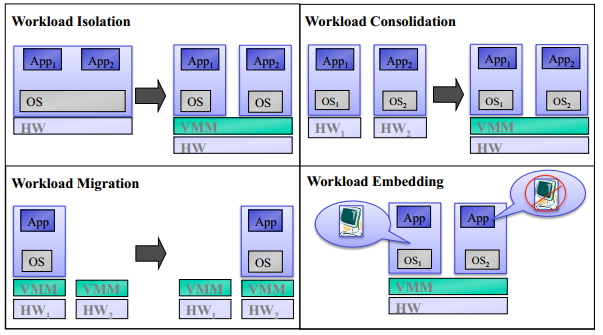
\includegraphics[width=0.7\linewidth]{fig/vorteile-hypervisor-virtualisierung}
\caption{Vorteile Hypervisor Virtualisierung}
\label{fig:vorteile-hypervisor-virtualisierung}
\end{figure}

\subsection{Challenges beim Betrieb einer VMM}
\begin{itemize}
	\item BS und APP wissen nicht, dass eine VMM existiert.
	\item VMM sollte SW Stack gegenüber anderen VMs isolieren.
	\item VMM sollte vor allen anderen Gast-SW geschützt laufen.
	\item VMM sollte eine ''virtuelle Plattform Interface'' zu den Gast-SW präsentieren.
\end{itemize}


\subsection{X86-Virtualisierung}

\subsection{HW-Virtualisierung}

\section{Memory-Virtualisierung}
Physikalisch mapped das OS virtual Page Number zu physical Page Number. Eine VM denkt, dass es physisches Memory vor sich hat und kann so agieren. Aber dieses Memory wird durch den Hypervisor verwaltet. Das gesamte Memory der Maschine wird durch alle VMs geteilt. Der Dreh- und Angelpunkt ist der Hypervisor.

\subsection{Memory Verbrauch}
Man kann mit folgenden Möglichkeiten Memory sparen, auch bekannt als Memory Rückgewinnungstechnologien:
\begin{description}
	\item[Page Sharing] In homogenen Gast Systemen findet sich viele identische Pages.
	\item[Page Patching] ''Fast gleiche'' Pages gibt es sehr viele.
	\item[Page Compression] Viele Pages die in naher Zukunft nicht verwendet werden.
	\item[Balloning] Wenn das Memory knapp wird
\end{description}


\section{Fragen}

\subsection{Der Studierende kennt die technische Grundlage wie Server Virtualisierung implementiert ist.}

\subsection{Der Studierende kennt Vor-/Nachteile der virtuellen Maschine}

\subsection{Der Studierende kann sein Erlerntes anwenden auf den Unterhalte und Betrieb eines Datencenters.}